\documentclass[12pt,a4paper]{article}
\usepackage[utf8]{inputenc}
\usepackage[spanish,es-tabla]{babel}
\usepackage{geometry}
\usepackage{graphicx}
\usepackage{multirow}
\usepackage{tabularx}
\usepackage{mathptmx}
\usepackage{fancyhdr}
\usepackage{array}
\usepackage[table]{xcolor}
\usepackage{titlesec}
\usepackage{setspace}
\usepackage{microtype}
\usepackage{lastpage}
\usepackage{booktabs}
\usepackage{enumitem}
\usepackage{amsmath}
\usepackage{amsfonts}
\usepackage{amssymb}

\graphicspath{{images/}{../images/}{../../images/}{./}}

\geometry{
    top=4.7cm,
    bottom=2.5cm,
    left=2.5cm,
    right=2.5cm,
    headheight=3.9cm,
    headsep=0.4cm
}

\setstretch{1.15}
\setlength{\parindent}{0pt}
\setlength{\parskip}{0.45em}
\setlength{\tabcolsep}{4pt}

\titleformat{\section}
  {\normalfont\fontsize{12}{14.5}\bfseries}{\thesection.}{0.6em}{\uppercase}
\titlespacing*{\section}
  {0pt}{1.8ex plus 0.4ex minus 0.2ex}{0.6ex plus 0.2ex}

\titleformat{\subsection}
  {\normalfont\fontsize{11.5}{13.5}\bfseries}{\thesubsection.}{0.5em}{}
\titlespacing*{\subsection}
  {0pt}{1.4ex plus 0.3ex minus 0.1ex}{0.4ex plus 0.1ex}

\titleformat{\subsubsection}
  {\normalfont\fontsize{10.5}{12.5}\bfseries\itshape}{\thesubsubsection.}{0.4em}{}
\titlespacing*{\subsubsection}
  {0pt}{1.1ex plus 0.2ex minus 0.1ex}{0.3ex plus 0.1ex}

\newcolumntype{Y}{>{\centering\arraybackslash}X}
\newcolumntype{L}{>{\raggedright\arraybackslash}X}
\newcolumntype{C}{>{\centering\arraybackslash}X}

\definecolor{headerred}{RGB}{180, 0, 0}
\definecolor{darkred}{RGB}{140, 0, 0}
\definecolor{lightgraybg}{RGB}{248, 248, 248}
\definecolor{tableheader}{RGB}{232, 238, 246}

\newcommand{\docCodigo}{TI-SIGE-ENT-S4-001}
\newcommand{\docVersion}{1.0}
\newcommand{\docProceso}{DESARROLLO FRONTEND / WIZARD Y EXPERIENCIA DE USUARIO}
\newcommand{\docElaboracion}{16/09/2026}
\newcommand{\docRevision}{EN PROGRESO AVANZADO}
\newcommand{\docTitulo}{LAYOUT DEL WIZARD MODULAR EN PESTAÑAS (FRONTEND)}
\newcommand{\docOrganizacion}{FACULTAD DE INGENIERÍA EN SISTEMAS, ELECTRÓNICA E INDUSTRIAL}
\newcommand{\docSubOrganizacion}{CARRERA DE INGENIERÍA DE SOFTWARE}

\newcommand{\encabezadofrecuente}{%
    \renewcommand{\arraystretch}{1.15}%
    \noindent\makebox[\textwidth][c]{%
    \begin{tabularx}{\textwidth}{|>{\centering\arraybackslash}m{2.8cm}|Y|>{\centering\arraybackslash}m{4.8cm}|}
        \hline
        \multirow{4}{2.8cm}{\centering\raisebox{-1.15cm}{
\includegraphics[width=2.5cm,height=2.0cm,keepaspectratio]{logo.png}}}
        & \textbf{\fontsize{9}{11}\selectfont \docOrganizacion} 
        & \textbf{\fontsize{8}{10}\selectfont CÓDIGO:} \fontsize{8}{10}\selectfont \docCodigo \\
        \cline{3-3}
        & \textbf{\fontsize{8.5}{10.5}\selectfont \docSubOrganizacion} 
        & \textbf{\fontsize{8}{10}\selectfont VERSIÓN:} \fontsize{8}{10}\selectfont \docVersion \\
        \cline{2-3}
        & \textbf{\fontsize{8}{10}\selectfont PROCESO:} \fontsize{8}{10}\selectfont \docProceso 
        & \textbf{\fontsize{8}{10}\selectfont ELABORACIÓN:} \fontsize{8}{10}\selectfont \docElaboracion \\
        \cline{2-3}
        & \textbf{\fontsize{8.5}{10.5}\selectfont \docTitulo} 
        & \textbf{\fontsize{8}{10}\selectfont ÚLTIMA REVISIÓN:} \fontsize{8}{10}\selectfont \textbf{\textcolor{darkred}{\docRevision}} \\
        \hline
    \end{tabularx}%
    }%
}

\pagestyle{fancy}
\fancyhf{}
\fancyhead[C]{\encabezadofrecuente}
\fancyfoot[C]{\fontsize{10}{12}\selectfont Página \thepage\ de \pageref{LastPage}}
\renewcommand{\headrulewidth}{0pt}

\begin{document}

\section{Título}
\textbf{Denominación del Entregable:} Desarrollo del Wizard Modular Asistido por Pasos para Elaboración de Planes e Informes

\vspace{0.15cm}
\noindent
\textbf{Ficha Técnica de Identificación:}
\begin{itemize}[leftmargin=1.5em, itemsep=1.5pt, topsep=1.5pt]
    \item \textbf{Código Documental:} \docCodigo \quad | \quad \textbf{Versión:} \docVersion
    \item \textbf{Institución:} Universidad Técnica de Ambato (UTA) -- FISEI
    \item \textbf{Carrera:} Ingeniería de Software (Séptimo Semestre "A")
    \item \textbf{Módulo Académico:} Gestión de Proyectos de Software
    \item \textbf{Docente Tutor:} Ing. Paulo Torres
    \item \textbf{Fecha de Elaboración:} \docElaboracion \quad | \quad \textbf{Estado:} \textbf{\textcolor{darkred}{En Desarrollo / Semana 4 en Curso}}
    \item \textbf{Período de Ejecución:} Semana 4 (15/09/2026 al 18/09/2026 -- EDT 3.5: 4 días laborables, 32h)
\end{itemize}

\section{Introducción}
Los formatos institucionales del SGC (\texttt{UTA-SGC-A-2-1-P7-T1} para el Plan de Trabajo e \texttt{UTA-SGC-A-2-1-P7-T2} para el Informe de Cumplimiento) se componen de múltiples secciones secuenciales: Datos Informativos, Justificación/Objetivos, Matriz Cronograma de Actividades, Anexos/Evidencias y Circuito de Firmas. La presentación de estos formularios en un formato monolítico extenso satura al usuario y propicia la pérdida de información.

Para optimizar la interacción, se diseñó e implementó un componente asistido por pasos (**Wizard Modular**) en React 19. Este asistente divide el llenado en pestañas lógicas conectadas, valida los requisitos mínimos de cada etapa antes de permitir la navegación, proporciona un indicador de avance porcentual en tiempo real y gestiona el estado transaccional del expediente.

\section{Objetivo}

\subsection{Objetivo General}
Desarrollar el componente de interfaz \texttt{PlanEditorWizard.tsx} bajo la arquitectura de pestañas modulares en React 19, guiando al docente en el llenado guiado y secuencial de su planificación semestral conforme al formato oficial de la FISEI UTA.

\subsection{Objetivos Específicos}
\begin{itemize}[leftmargin=1.5em, itemsep=1.5pt, topsep=1.5pt]
    \item Diseñar la barra de navegación por pasos con estados visuales: *Completado*, *En Edición*, *Pendiente* y *Bloqueado*.
    \item Implementar validaciones deterministas de salida en cada pestaña (no permitir avanzar si faltan campos obligatorios).
    \item Integrar el cálculo reactivo del porcentaje de completitud global del expediente.
\end{itemize}

\section{Alcance}

\subsection{Alcance Incluido}
Pestaña 1 (Datos Informativos), Pestaña 2 (Justificación y Objetivos), Pestaña 3 (Contenedor de la Matriz de Actividades), Pestaña 4 (Anexos y Evidencias) y Pestaña 5 (Vista previa y Cascada de Firmas).

\subsection{Límites y Exclusiones}
El cálculo dinámico de fórmulas de ponderación se encapsula en EDT 3.9.

\section{Definiciones}
\begin{itemize}[leftmargin=1.5em, itemsep=2pt, topsep=2pt]
    \item \textbf{Wizard Pattern:} Patrón de diseño de interfaz que descompone una tarea compleja en pasos individuales secuenciales.
    \item \textbf{Completitud Reactiva:} Cálculo en memoria del progreso del formulario que se actualiza con cada cambio de entrada.
\end{itemize}

\section{Responsabilidades}
\begin{itemize}[leftmargin=1.5em, itemsep=2pt, topsep=2pt]
    \item \textbf{Andrea Vasquez (Frontend / QA):} Programación de componentes React, manejo de estado y validadores de pestañas.
    \item \textbf{Heidy Villavicencio (Analista / UI-UX):} Ajuste estético, iconos de estado y pruebas de usabilidad según wireframes.
    \item \textbf{Ing. Paulo Torres (Docente Tutor):} Supervisión técnica y validación del diseño UX.
\end{itemize}

\section{Método, Políticas y Contenidos}
Construcción de componentes desacoplados en React 19 con TypeScript estricto y React Hook Form. Se definen políticas estrictas de navegación: el usuario puede retornar a pasos anteriores ya guardados, pero se restringe el avance a etapas subsiguientes si el paso activo contiene errores de validación.

\begin{figure}[htbp]
    \centering
    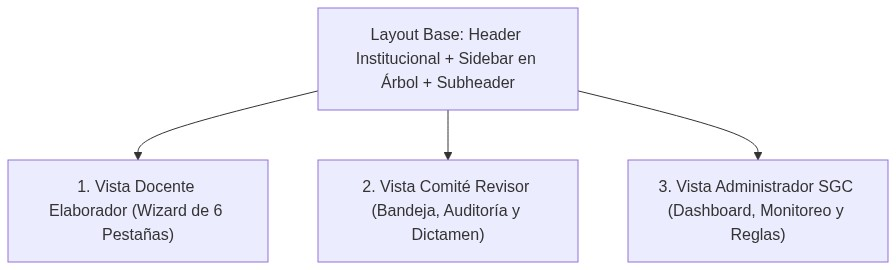
\includegraphics[width=0.88\textwidth,keepaspectratio]{images/s2_05_layout_vistas.png}
    \caption{Distribución en Pestañas Modulares del Asistente Wizard en SIGE.}
    \label{fig:layout_vistas}
\end{figure}

\section{Descripción de actividades}

\subsection{Estructura de Pasos del Wizard Modular}
El formulario se divide en 5 pestañas secuenciales claramente delimitadas:
\begin{enumerate}[leftmargin=1.5em, itemsep=2pt]
    \item \textbf{Datos Informativos:} Período, docente, dedicación horaria y carrera.
    \item \textbf{Justificación y Objetivos:} Metas estratégicas del período.
    \item \textbf{Matriz de Actividades y Ponderaciones:} Tabla interactiva con validación al 100.00\%.
    \item \textbf{Anexos y Evidencias:} Repositorio de medios de verificación en MinIO S3.
    \item \textbf{Cascada de Firmas:} Vista previa de foliación y circuito secuencial de legalización.
\end{enumerate}

\subsection{Flujo de Validación y Completitud Reactiva}
El avance porcentual se calcula reactivamente en memoria:
\begin{equation}
\text{Progreso Global} = \frac{\sum_{i=1}^{5} \text{PuntajePaso}_i}{5} \times 100\%
\end{equation}
Si el docente intenta acceder a la pestaña de Firmas sin alcanzar el 100\% de ponderación en la Matriz, la interfaz despliega una alerta modal bloqueante con la advertencia de Validation Gate.

\subsection{Conclusiones y Recomendaciones Técnicas}
\begin{itemize}[leftmargin=1.5em, itemsep=2pt]
    \item El Wizard modular elimina la fricción de los formatos Word estáticos, reduciendo los errores por omisión de datos obligatorios.
    \item La arquitectura por componentes facilita el mantenimiento y la reutilización tanto para el Plan de Trabajo como para el Informe de Cumplimiento.
    \item Conectar el Wizard con el servicio de autoguardado en segundo plano desarrollado en EDT 4.2 para evitar pérdidas accidentales de texto.
\end{itemize}

\vspace{0.3cm}

% =============================================================
% 10. FIRMAS DE RESPONSABILIDAD
% =============================================================
\section{Firmas de Responsabilidad}

\noindent
\renewcommand{\arraystretch}{1.2}
\begin{tabularx}{\textwidth}{|>{\raggedright\arraybackslash}m{2.9cm}|>{\raggedright\arraybackslash}X|>{\centering\arraybackslash}m{4.6cm}|>{\centering\arraybackslash}m{2.3cm}|}
    \hline
    \rowcolor{headerred}
    \textcolor{white}{\textbf{ACCIÓN}} & \textcolor{white}{\textbf{NOMBRE Y CARGO}} & \textcolor{white}{\textbf{FIRMA}} & \textcolor{white}{\textbf{FECHA}} \\
    \hline
    \textbf{Elaborado por:} & Andrea Vasquez\newline \textit{Frontend Developer / QA} & \parbox[c]{4.4cm}{\centering\vspace{10pt}\textbf{\textcolor{blue!80}{\scriptsize [ FIRMADO DIGITALMENTE ]}}\vspace{10pt}} & 16/09/2026 \\
    \hline
    \textbf{Revisado por:} & Heidy Villavicencio\newline \textit{Analista de Requerimientos / UI-UX} & \parbox[c]{4.4cm}{\centering\vspace{4pt}
\includegraphics[height=1.5cm,width=4.0cm,keepaspectratio]{images/firma_heidi.png}\vspace{4pt}} & 16/09/2026 \\
    \hline
    \textbf{Aprobado por:} & Ing. Paulo Torres\newline \textit{Docente Tutor - Gestión Proyectos Software} & \parbox[c]{4.4cm}{\centering\vspace{10pt}\textbf{\textcolor{gray!80}{\scriptsize [ PENDIENTE DE APROBACIÓN ]}}\vspace{10pt}} & \textbf{\textcolor{gray!90}{Pendiente}} \\
    \hline
\end{tabularx}

\vspace{0.4cm}

% =============================================================
% 11. CONTROL DE CAMBIOS
% =============================================================
\section{Control de Cambios}

\noindent
\renewcommand{\arraystretch}{1.2}
\begin{tabularx}{\textwidth}{|>{\hsize=0.45\hsize\centering\arraybackslash}X|>{\hsize=1.55\hsize\raggedright\arraybackslash}X|>{\hsize=1.2\hsize\raggedright\arraybackslash}X|>{\hsize=0.8\hsize\centering\arraybackslash}X|}
    \hline
    \rowcolor{gray!20}
    \textbf{Versión} & \textbf{Descripción del cambio} & \textbf{Responsable del cambio} & \textbf{Fecha de aprobación} \\
    \hline
    1.0 & Creación del componente Wizard modular de 5 pestañas para Séptimo Semestre "A" & Andrea Vasquez & 16/09/2026 \\
    \hline
\end{tabularx}

\vspace{0.4cm}

% =============================================================
% 12. ANEXOS
% =============================================================
\section{Anexos}

\subsection*{Anexo 1: Referencias Bibliográficas}
\begin{itemize}[leftmargin=1.5em, itemsep=2pt]
    \item Nielsen Norman Group. (2024). \textit{Wizards: Definition and Design Recommendations}.
    \item React Community. (2026). \textit{React 19 Hooks and Component State}.
\end{itemize}

\subsection*{Anexo 2: Flujo Lógico de Validación por Pasos}
Matriz de dependencias y condiciones de salida requeridas en cada pestaña antes de habilitar el botón de avance secuencial.

\end{document}


